\documentclass[a4paper]{article}
\usepackage{float}
\usepackage{fullpage}
\usepackage{amsmath}
\usepackage{amssymb}
\usepackage{graphicx}
\usepackage{hyperref}
\usepackage{listings}
\usepackage{xcolor}

\numberwithin{equation}{section}

\title{Pivoting Rules for the Simplex Method: Implementation, Complexity and Run-Time Scaling}
\author{Kevin He}
\date{April 2025}

\begin{document}

\maketitle


\section{Python codes}
\label{sec:code}

\subsection{Code for \texttt{find\_pivot\_largest\_subscript}}\label{sec:code_ls}

\begin{lstlisting}[language=Python,numbers=left,numbersep=5pt]
def find_pivot_largest_subscript(tableau):
    """
    Using the largest subscript rule (opposite of Bland's rule) and the
    minimum ratio test, find the pivot entry in the tableau.

    Parameters
    ----------
    tableau : array
        The simplex method tableau in basic form

    Returns
    -------
    final_r, final_s : integer
        Row and column indexes of the pivot

    Notes
    -----
    Assumes that there is a negative reduced cost that we can pivot on.
    """
    M, N = tableau.shape
    m = M-1
    n = N-1

    # Largest subscript rule: find the last negative reduced cost
    final_s = n
    while final_s >= 1 and tableau[0, final_s] >= 0:
        final_s -= 1

    # Minimum ratio test plus largest subscript rule
    final_r = 0
    theta_star = np.inf
    for i in range(1, m+1):
        if tableau[i, final_s] > 0:
            if tableau[i, 0] / tableau[i, final_s] < theta_star:
                final_r = i
                theta_star = tableau[i, 0] / tableau[i, final_s]

    return final_r, final_s
\end{lstlisting}



\subsection{Code for \texttt{find\_pivot\_largest\_coefficient}}
\label{sec:code_lc}


\begin{lstlisting}[language=Python,numbers=left,numbersep=5pt]
def find_pivot_largest_coefficient(tableau):
    """
    Using the largest coefficient rule and the minimum ratio test,
    find the pivot entry in the tableau.

    Parameters
    ----------
    tableau : array
        The simplex method tableau in basic form

    Returns
    -------
    final_r, final_s : integer
        Row and column indexes of the pivot

    Notes
    -----
    Assumes that there is a negative reduced cost that we can pivot on.
    """
    M, N = tableau.shape
    m = M-1
    n = N-1

    # Largest coefficient rule: find the MOST negative reduced cost
    final_s = -1
    most_negative = 0
    for s in range(1, n+1):
        if tableau[0, s] < most_negative:
            most_negative = tableau[0, s]
            final_s = s

    # Minimum ratio test plus largest coefficient rule
    final_r = 0
    theta_star = np.inf
    for i in range(1, m+1):
        if tableau[i, final_s] > 0:
            if tableau[i, 0] / tableau[i, final_s] < theta_star:
                final_r = i
                theta_star = tableau[i, 0] / tableau[i, final_s]

    return final_r, final_s
\end{lstlisting}


\section{Complexity analysis}
\label{sec:complexity}

\subsection{Complexity of  \texttt{find\_pivot\_largest\_subscript}}
\label{sec:complexity_ls}


Example adopting the previous code in section~\ref{sec:code_ls}.

\begin{itemize}
  \item Initial setup: lines 19 to 21, take $\mathcal{O}(1)$.
  %
  \item Column selection: Worst case, lines 24 to 26 are used $\mathcal{O}(n)$ times as every column from right to left is examined. In each iteration:
  %
  \begin{itemize}
    \item   two comparisons: each $\mathcal{O}(1)$,
    \item and one decrement, $\mathcal{O}(1)$, is completed.

  \end{itemize}
  %
    Overall, lines 24 to 26 take $\mathcal{O}(1)$ * n =  $\mathcal{O}(n)$.
  %
  \item Row selection: lines 29 to 35, take in each iteration:
  %
\begin{itemize}
\item one comparison: $\mathcal{O}(1)$,
\item and one division: $\mathcal{O}(1)$.
\end{itemize}
  %
    Overall, lines 29 to 35 take $\mathcal{O}(1)$ * m = $\mathcal{O}(m)$ where m is the number of rows.
\end{itemize}

  Overall, we have a complexity of:
\begin{equation}
    \label{eq:complexity_ls}
  \mathcal{O}(1) + \mathcal{O}(n) + \mathcal{O}(m) = \mathcal{O}(n + m).
\end{equation}


\subsection{Complexity of  \texttt{find\_pivot\_largest\_coefficient}}
\label{sec:complexity_lc}

Example adopting the previous code in section~\ref{sec:code_lc}.

\begin{itemize}
  \item Initial setup: lines 20 to 22, take $\mathcal{O}(1)$.
  %
  \item Column selection: Worst case, lines 25 to 30 are used $\mathcal{O}(n)$ times as every column from right to left is examined. In each iteration:
  %
  \begin{itemize}
    \item   a comparison:  $\mathcal{O}(1)$,
    \item and a possible assignment, $\mathcal{O}(1)$, is completed.

  \end{itemize}
  %
    Overall, lines 27 to 30 take $\mathcal{O}(1)$ * n =  $\mathcal{O}(n)$.
  %
  \item Row selection: lines 35 to 39, take in each iteration:
  %
\begin{itemize}
\item  two comparison: $\mathcal{O}(1)$,
\item and a possible division: $\mathcal{O}(1)$.
\end{itemize}
  %
    Overall, lines 35 to 39 take $\mathcal{O}(1)$ * m = $\mathcal{O}(m)$ where m is the number of rows.
\end{itemize}

  Overall, we have a complexity of:
\begin{equation}
    \label{eq:complexity_lc}
  \mathcal{O}(1) + \mathcal{O}(n) + \mathcal{O}(m) = \mathcal{O}(n + m).
\end{equation}


\section{Excel analysis}
\label{sec:excel}


Below are tables containing the $p_{0,1}$ for the averages and the worst cases for each of the pivoting rules from figures 1 and 2 (which can be found at the end of the report) given that $\log(t) = p_{0} \log(n) + p_{1}$.
\begin{table}[H]
  \caption{Table of $p_{0,1}$ for the averages for each of the pivoting rules (from figure 1)}
  \begin{center}
    \begin{tabular}{c|rrr}
      Coefficients& log(Bland)& log(Largest Subscript)& log(Largest Coefficient)\\
      \hline
      $p_0$& 1.456256887& 1.425344791& 1.19639858\\
      $p_1$& -4.953188932& -4.917116201& -4.874391443\\
    \end{tabular}
  \end{center}
\label{tab:average}
\end{table}
\begin{table}[H]
  \caption{Table of $p_{0,1}$ for the worst cases for each of the pivoting rules (from figure 2)}
  \begin{center}
    \begin{tabular}{c|rrr}
      Coefficients& log(Bland)& log(Largest Subscript)& log(Largest Coefficient)\\
      \hline
      $p_0$& 1.340340616& 1.419909531& 1.109457858\\
      $p_1$& -4.202956289& -4.429689972& -4.326703896\\
    \end{tabular}
  \end{center}
\label{tab:worst}
\end{table}

\section{Efficiency}
\label{sec:efficiency}


The time complexity analysis shows that the largest subscript and the largest coefficient rules have the same total time complexity of $\mathcal{O}(m+n)$, suggesting that they should perform similarly. However, the largest coefficient rule tends to be more efficient on average, as shown by its smaller $p_0$ value (1.196 (3 decimal places)) compared to the largest subscript rule (1.425) and Bland's rule (1.456) as shown in Table 1. This suggests that the largest coefficient rule scales better with instance size, as run time does not increase as much as the other two pivoting rules when the instance size increases. In addition to this, when considering worst case run times, the largest subscript rule has a higher $p_0$ (1.420 (to 3 decimal places)) compared to the largest coefficient rule (1.109). In conclusion, the largest coefficient rule is generally more efficient and scales better compared to Bland's rule and the largest subscript rule.


\begin{figure}[h!]
  \begin{center}
    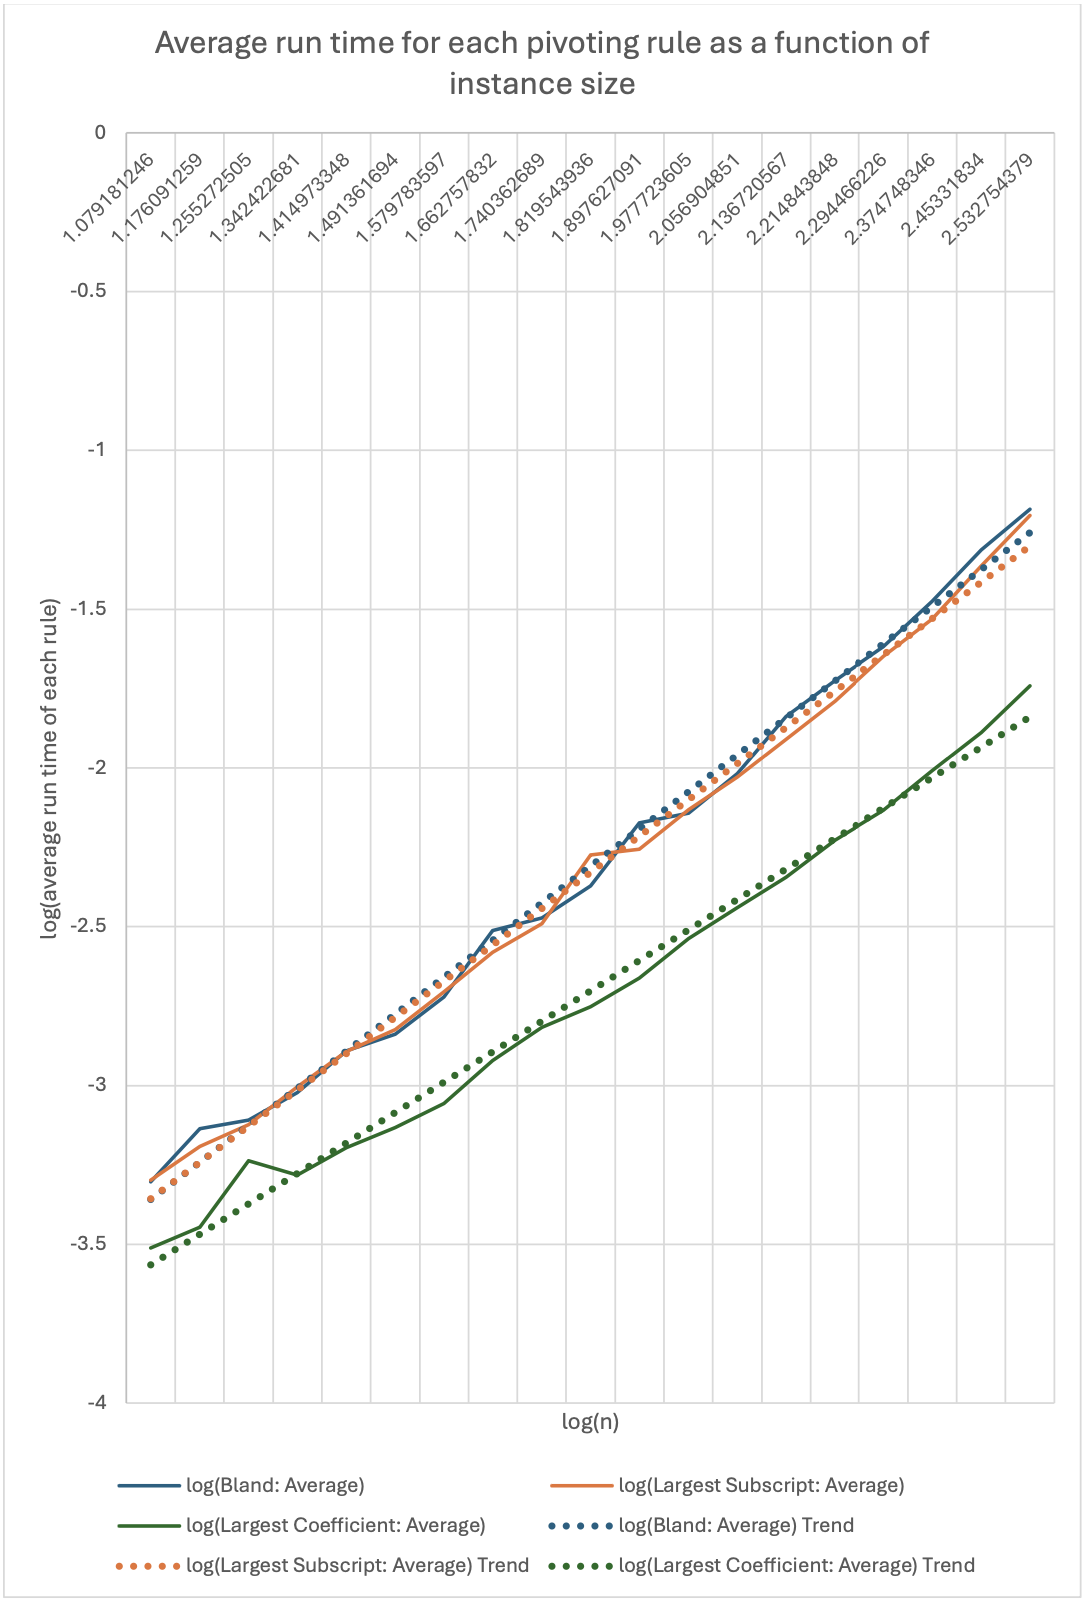
\includegraphics[width=0.7\textwidth]{figures/average_runtime.png}
  \end{center}
  \caption{ The Average run time for each pivoting rule as a function of instance size.
  }
  \label{fig:average}
\end{figure}
\begin{figure}[h!]
  \begin{center}
    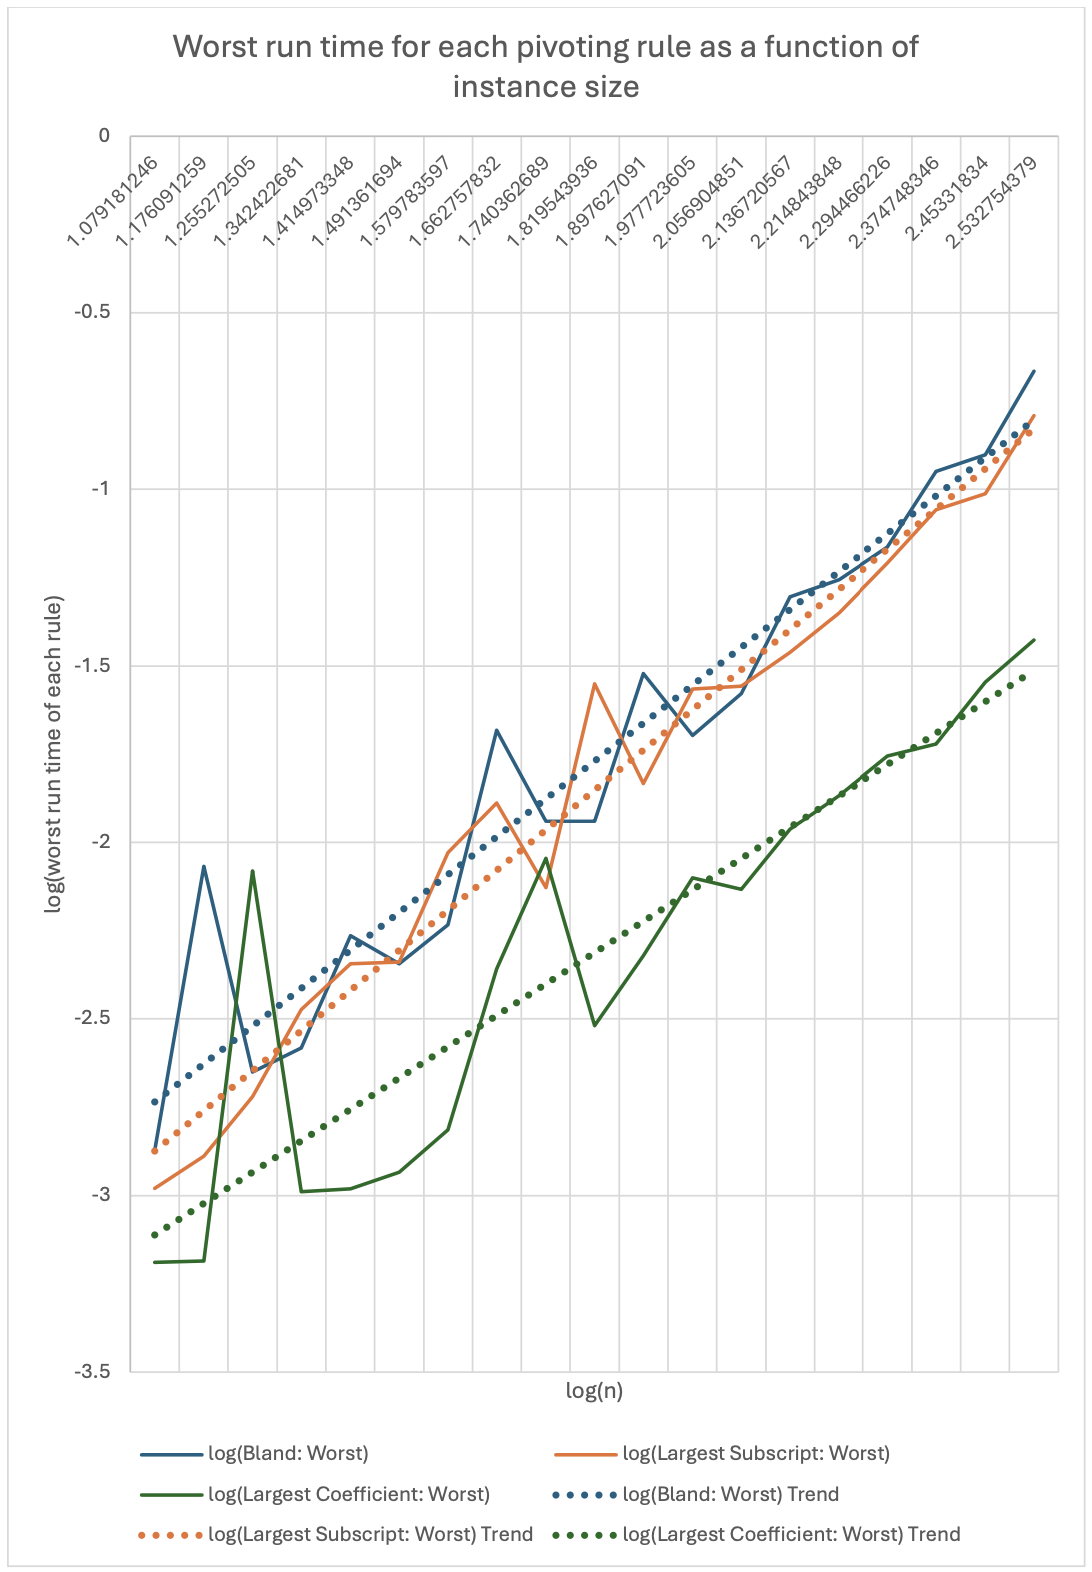
\includegraphics[width=0.7\textwidth]{figures/worst_case_runtime.png}
  \end{center}
  \caption{ The Worst case run time for each pivoting rule as a function of instance size.
  }
  \label{fig:worst}
\end{figure}
\end{document}
